\documentclass[UTF8,10.5pt,a4paper]{ctexart}

\usepackage{amsmath,amsthm,amsfonts,amssymb,amscd}
\usepackage{latexsym}
\usepackage{amsmath}
\usepackage{amsthm}
\usepackage{amsfonts}
\usepackage{caption2}     %修改图片表格名称字体字号的宏包
\usepackage{float}        %自己设置图片插入位置
\usepackage{fancyhdr}     %设置页眉页脚的宏包
\usepackage{graphicx}     %插入图片
\usepackage{lastpage}     %引用最后一页
\graphicspath{{figures/}} %%图片路径
%% TODO: geometry
\usepackage[top=3.2cm,bottom=3.8cm,left=3.3cm,right=1.8cm]{geometry}  %设置页边距
%% TODO: zhuang ding xian
\usepackage{fancybox}                      %画边界线
\fancyput*(-0.8cm,-4.3cm){$|$}%
\fancyput*(-0.8cm,-4.9cm){$|$}%
\fancyput*(-0.8cm,-5.5cm){$|$}%
\fancyput*(-0.8cm,-6.1cm){$|$}%
\fancyput*(-0.8cm,-6.7cm){$|$}%
\fancyput*(-0.8cm,-7.3cm){$|$}%
\fancyput*(-0.8cm,-7.9cm){$|$}%
\fancyput*(-0.8cm,-8.5cm){$|$}%
\fancyput*(-0.8cm,-9.1cm){$|$}%
\fancyput*(-0.8cm,-9.7cm){$|$}%
\fancyput*(-1.0cm,-10.3cm){装}%
\fancyput*(-0.8cm,-10.9cm){$|$}%
\fancyput*(-0.8cm,-11.5cm){$|$}%
\fancyput*(-0.8cm,-12.1cm){$|$}%
\fancyput*(-0.8cm,-12.7cm){$|$}%
\fancyput*(-0.8cm,-13.3cm){$|$}%
\fancyput*(-1.0cm,-13.9cm){订}%
\fancyput*(-0.8cm,-14.5cm){$|$}%
\fancyput*(-0.8cm,-15.1cm){$|$}%
\fancyput*(-0.8cm,-15.7cm){$|$}%
\fancyput*(-0.8cm,-16.3cm){$|$}%
\fancyput*(-0.8cm,-16.9cm){$|$}%
\fancyput*(-1.0cm,-17.5cm){线}%
\fancyput*(-0.8cm,-18.1cm){$|$}%
\fancyput*(-0.8cm,-18.7cm){$|$}%
\fancyput*(-0.8cm,-19.3cm){$|$}%
\fancyput*(-0.8cm,-19.9cm){$|$}%
\fancyput*(-0.8cm,-20.5cm){$|$}%
\fancyput*(-0.8cm,-21.1cm){$|$}%
\fancyput*(-0.8cm,-21.7cm){$|$}%
\fancyput*(-0.8cm,-22.3cm){$|$}%
\fancyput*(-0.8cm,-22.9cm){$|$}%
\fancyput*(-0.8cm,-23.5cm){$|$}%

%% TODO: toc
%设置目录格式(引文部分)
\usepackage[titles]{tocloft}
\renewcommand{\cftdot}{$\cdot$}
\renewcommand{\cftdotsep}{1}
\setlength{\cftbeforesecskip}{10pt}
\setlength{\cftbeforesubsecskip}{3pt}
\setlength{\cftbeforesubsubsecskip}{0pt}
\renewcommand{\cftsecfont}{\zihao{5}\heiti}
\renewcommand{\cftsubsecfont}{\zihao{5}\heiti}
\renewcommand{\cftsubsubsecfont}{\zihao{5}\heiti}
\renewcommand{\cftsecleader}{\cftdotfill{\cftsecdotsep}}
\renewcommand{\cftsecdotsep}{\cftdotsep}
\renewcommand{\cftsecpagefont}{\zihao{5}}
\renewcommand{\cftsubsecpagefont}{\zihao{5}}
\renewcommand{\cftsubsubsecpagefont}{\zihao{5}}
%% TODO: equation numbering
\numberwithin{equation}{section}

%% TODO: theorem
%设置定理定义等的格式,如果某项的编号是跟着章节的,在后面加[section]
\theoremstyle{definition}
\newtheorem{thm}{定理\hspace{0.05pt}}[section]
\newtheorem{cor}{推论\hspace{0.05pt}}[section]
\newtheorem{lem}{引理\hspace{0.05pt}}[section]
\newtheorem{prop}{命题\hspace{0.05pt}}[section]
\newtheorem{conj}{猜想\hspace{0.05pt}}

\theoremstyle{definition}
\newtheorem{dfn}{定义\hspace{0.05pt}}[section]
\newtheorem{exmp}{例\hspace{0.05pt}}[section]
\newtheorem{rem}{注\hspace{0.05pt}}
%\newtheorem{note}[thm]{Note}
\newtheorem*{pf}{证明}

%% TODO: numbering of floats

%设置图表编号和章节相关联,参见http://blog.sina.com.cn/s/blog_5e16f1770100h6ts.html
\usepackage[T1]{fontenc}
%\usepackage[utf8]{inputenc}
%\usepackage[font=small,labelfont={bf,sf},tableposition=top]{caption}

\makeatletter
\renewcommand{\thefigure}{\ifnum \c@section>\z@ \thesection.\fi \@arabic\c@figure}
\renewcommand{\thetable}{\ifnum \c@section>\z@ \thesection.\fi \@arabic\c@table}
\makeatother


%\bibliographystyle{plainnat}
%\begin{CJK*}{GBK}{song}
%\title{}
%\author{}
%\date{}

%\CJKindent
\begin{document}


% TODO: title page

%% TODO: pagestyle
\linespread{1.5}  %1.5倍行距
\pagestyle{fancy} %页眉页脚设置
\fancyhead{}      %清空默认页眉
\fancyfoot{}      %清空默认页脚
\fancyhead[L]{\qquad 
\includegraphics[height=1.34cm]{tongji}}   %页眉左侧插入同济大学logo
\fancyhead[R]{\large 毕业设计(论文)~\\}
\fancyfoot[LE,RO]{{\large 共\quad \pageref{LastPage}\quad 页\quad 第\quad \thepage \quad 页}} %偶数页左侧(LE),奇数页右侧(RO)标页码,oneside打印只用写RO
\renewcommand{\headrulewidth}{1.5pt}  %页眉横线
\renewcommand{\footrulewidth}{1.5pt}
%\newgeometry{} 单独调节某页边距
%\maketitle
\thispagestyle{fancy}


%% TODO: title
~\\
\begin{center}\heiti\zihao{2}
经典力学的数学基础
\end{center}
%% TODO: abstract
\begin{center}\heiti\zihao{4}
    摘\quad 要
\end{center}
\hspace{2mm}
 {\heiti\zihao{-5}}\quad {\songti\zihao{-5}历史上,数学与物理一直有密不可分的联系,许多数学理论发展自物理问题,很多数学方法和工具也都在物理学中找到实际应用.本文以经典力学为研究范畴,用数学语言叙述了其中的重要原理和定理,如三大守恒定律,最小作用量原理,诺特定理及刘维尔定理等等,体现了包括微分方程,变分法,守恒律,微分流形,辛结构在内的各种抽象数学工具和概念如何帮助我们描述和求解现实中的力学问题.根据经典力学的不同表述,文章主体分为牛顿力学,拉格朗日力学,以及哈密顿力学三章,每部分内又可分为运动方程的推导,相空间的几何,不变量的导出三部分,并附有实例说明如何通过守恒律简化方程求解.
}
%局部修改字体字号{\字体名\zihao{} ...}
%% TODO: keywords
\par
\vskip 5mm
\noindent {\heiti\zihao{5}关键词:}\quad{\songti\zihao{-5}  经典力学, \quad 微分方程, \quad 微分流形, \quad 守恒律}~\\


\newpage

% TODO: english title page

%\thispagestyle{fancy}
\vskip 4mm
%% TODO: english title
\begin{center}\heiti\zihao{2}
	{\bf {English Title} }
\end{center}
%% TODO: english abstract
\begin{center}\heiti\zihao{4}
\bf{	ABSTRACT}
\end{center}
\hspace{2mm}
 {\heiti\zihao{-5}}\quad {\songti\zihao{-5}Historically, mathematics and physics have been inextricably linked, since many mathematical theories were inspired by physical problems and a variety of mathematical tools find applications in physical areas. In this paper,key principles and theorems about classical mechanics are discussed using mathematical language, such as the conservation law,Hamilton least action principle, Noether's theorem and Liouville's theorem. This paper also tries to show that how does the abstract mathematical tools help us describe and solve practical mechanics problems. Among those mathematical tools are variational principles, differential equations and differential manifolds. The body of this paper is divided into three sections according to the different interpretations of classical mechanics. And within each section, we will present an introduction to the equations of motion and the geometry of phase space. We also give the derivation of some key invariants. Examples showing how to simplify the equations by conservation laws are attached as well.
}\par

%% TODO: english keywords
\vskip 4mm
\noindent{\heiti\zihao{5}\bf {Key\ words:}}\quad
{\songti\zihao{-5} Classical Mechanics, \quad Differential Equations, \quad Differential Manifolds,
	\quad Conservation Laws}
\par

%% TODO: table of contents

%以下为修改目录格式的正文内语句,正文内用@命令需用\makeatletter,\makeatother括起来
\renewcommand{\contentsname}{\centerline{目\quad 录}}
\makeatletter
\renewcommand{\numberline}[1]{%
\settowidth\@tempdimb{#1\hspace{0.5em}}%
\ifdim\@tempdima<\@tempdimb%
\@tempdima=\@tempdimb%
\fi%
\hb@xt@\@tempdima{\@cftbsnum #1\@cftasnum\hfil}\@cftasnumb}
\makeatother

\newpage
\tableofcontents   %放置目录
\newpage

%% TODO: title style of headings

%以下两段修改章节标题格式,参数含义见博客http://blog.sina.com.cn/s/blog_5e16f1770100lqn7.html
\makeatletter
\renewcommand\subsubsection{\@startsection{subsubsection}{3}{2em}%
{2.3ex \@plus -1ex \@minus -.2ex}%
{2.3ex \@plus.2ex}%
{\normalfont\normalsize\bfseries}}
\makeatother
\makeatletter
\renewcommand\subsection{\@startsection{subsection}{2}{0em}%
{2.3ex \@plus -1ex \@minus -.2ex}%
{2.3ex \@plus.2ex}%
{\normalfont\normalsize\bfseries}}
\makeatother




\section{绪论}

经典力学是力学的一个分支,主要研究宏观世界和低速状态下的物体运动.
\par 经典力学最初的表达形式由牛顿给出,牛顿力学以质点作为研究对象,以三维欧氏空间为构型空间,它着重分析力、动量、速度、加速度、角动量、力矩等物理量,在处理质点系统问题时,强调分别对单个质点进行受力分析,然后来推断整个质点系统的运动状态.用牛顿力学处理简单问题时,解题方式简单直接,且非常直观.但实际力学系统往往存在约束,而约束力又取决于运动情况,它们常作为未知量出现于运动方程中.牛顿方式对于受约束的力学系统并不方便,因为用它求解带约束系统的问题常需要知道约束的显式表达,很多时候这点难以做到.在牛顿力学中,约束越多,就需要引入更多的方程来表示这些约束,问题会越来越复杂.牛顿力学的这些缺陷促使物理学家和数学家们思考新的力学系表述方式.除此之外,研究光、电磁场、微观粒子等物理现象时,整个牛顿力学的基本观念都受到了挑战.在人们不得不承认新的物理事实——相对论效应,波粒二象性等之后,就需要在经典力学理论中寻找这样一种理论,它能较顺利地超越经典概念的束缚,自然地跳向非经典力学——相对论力学、量子力学等.
\par 分析力学是数学、力学研究者为克服上述困难所取得的成果的一部分,在一定程度上解决了上述问题.它给出了力学系统在完全一般性的广义坐标下具有不变形式的动力学方程组,并突出了能量函数的意义.分析力学概括了比牛顿力学广泛得多的系统, 分析力学的数学形式有着极好的性质, 它不仅提供了解决天体力学及一系列动力学问题的较佳途径, 同时给量子力学的发展提供了启示, 最适于成为引向现代物理的跳板. 其最小作用量原理提供了建立相对论力学和量子力学最简练而富有概括性的出发点.
\par 拉格朗日在其名著《分析力学》中,在总结历史上各种力学基本原理的基础上,进一步把数学分析应用于质点和刚体力学,提出了运用于静力学和动力学的普遍方程,引进广义坐标的概念,建立了拉格朗日方程,把力学体系的运动方程丛以力为基本概念的牛顿形式,改变为以能量为基本概念的分析力学形式,奠定了分析力学的基础,为把力学理论推广应用到物理学其他领域开辟了道路.有了拉格朗日方程我们还可以给出诺特定理简单情形下的一个证明.诺特定理是物理学的中心理论,它揭示了系统连续对称性和守恒量之间的关系.拉格朗日还给出刚体在重力作用下,绕旋转对称轴上的定点转动(拉格朗日陀螺)的欧拉动力学方程的解,对三体问题的求解方法有重要贡献,解决了限制性三体运动的定型问题.拉格朗日对流体运动的理论也有重要贡献,提出了描述流体运动的拉格朗日方法.拉格朗日的研究工作中,约有一半同天体力学有关.他用自己在分析力学中的原理和公式,建立起各类天体的运动方程.在天体运动方程的解法中,拉格朗日发现了三体问题运动方程的五个特解,即拉格朗日平动解.此外,他还研究了彗星和小行星的摄动问题,提出了彗星起源假说等.
\par 爱尔兰物理学家哈密顿进一步发展了分析力学.他在于1833年发表的关于平稳作用量原理的表述中提出了哈密顿原理,这个原理说一个物理系统的拉格朗日函数所构成的泛函的变分问题的解可以表达这物理系统的动力行为.拉格朗日函数又称为拉格朗日量,包含了这物理系统所有的物理内涵.这泛函称为作用量.哈密顿原理提供了一种新的方法来表述物理系统的运动.不同于牛顿运动定律的微分方程方法,该方法以积分方程来设定系统的作用量,在作用量平稳的要求下,使用变分法来计算整个系统的运动方程.
虽然哈密顿原理本来是用来表述经典力学,这原理也可以应用于经典场,像电磁场或引力场,甚至可以延伸至量子场论等等.根据这一原理,力学与几何光学找到了相似之处.后来发现,哈密顿原理可推广到物理学的许多领域,如电磁学等. 他还给出了经典力学中又一种表述:哈密顿力学.在勒让德变换下,拉格朗日方程可转变为哈密顿方程.哈密顿方程不同于拉格朗日方程以广义坐标和广义速度为独立变量,它的独立变量是广义坐标和广义动量.在牛顿力学里速度与动量只相差一个质量,但在这里,广义速度是逆变向量,拉格朗日力学的状态空间为以构型空间为底空间的切丛;广义动量为协变向量,哈密顿力学的相空间为与切丛对偶的以构型空间为底空间的余切丛.相空间为哈密顿力学的重要研究对象,在相空间中一个重要的不变量是庞加莱积分不变量,庞加莱积分不变量在局部微分同胚下保持不变.这个性质在经典力学中对应正则变换,可以将一个哈密顿系统变换为另一个哈密顿系统,从而大大简化方程的求解,它在理论物理和天体力学中有重要应用.
\par 本文以阿诺德(Arnold)的名著《经典力学的数学方法》为蓝本,分别介绍了牛顿力学,拉格朗日力学,哈密顿力学的运动方程和与之相关的重要数学工具.文章主体按三种力学表述分为三部分,且以各系统的守恒律或者积分不变量为侧重点,描述了如何通过不变量来简化方程的求解.本文运用的数学方法主要有数学分析,变分法以及微分几何.
\newpage

\section{拉格朗日力学系}
\par 从本章开始本文跨入分析力学的范畴,本章将首先介绍变分原理,推导出拉格朗日方程,然后将构型空间从欧氏空间推广到微分流形上,并简要介绍诺特定理等拉格朗日系统中的重要结论.本章的讨论主要限于保守自制系统.

\subsection{理想完整约束系中的运动}
拉格朗日力学的一大优势就在于它简化了带有约束的力学系的处理,我们首先定义对带有约束的力学系进行定义.
\begin{dfn}
$\gamma$是质量为$(m_1,\ldots,m_n)$之质点组$(\textbf{r}_1,\ldots,\textbf{r}_n)$所组成的$3n$维构型空间里的$m$维曲面.令$\textbf{q}=(q_1,\ldots,q_m)$ 是$\gamma$上的某坐标表示,$\textbf{r}_i=\textbf{r}_i(\textbf{q})$.称以下方程表示的力学系为具有$3n-m$个理想完整约束的$n$质点力学系:
$$\frac{d}{dt}(\frac{\partial L}{\partial\dot{\textbf{q}}})=\frac{\partial L}{\partial\textbf{q}},\quad L=1/2\sum m_i\dot{\textbf{r}}_i^2-U(\textbf{q})$$
曲面$\gamma$称为约束力学系的构型空间.
\end{dfn}
一个具有约束的力学系的构形空间是一个微分流形.
\subsubsection{流形的基本概念}
本小节我们将给出关于微分流形的一系列基本事实,更详尽的叙述请见文献\cite{zzs}以及\cite{css}.
\begin{dfn}
设$M$是一个满足$T_2$,$C_2$公理的拓扑空间,$(U,\phi)$ 称为$M$的一个局部坐标或图卡,如果$U$是一个开集,$\phi$是从$U\text{到}\textbf{R}^m\text{的开集}\phi(U)$ 的同胚映射.$M$的两个图卡称为$C^\infty$相容的如果它们满足以下两种情形之一:
\begin{itemize}
     \item [(1)]$U\cap V=\emptyset\text{.}$
     \item [(2)]$U\cap V\neq\emptyset$且坐标变换$$\Psi\circ\Phi^{-1}:\Phi(U\cap V)\rightarrow\Psi(U\cap V)$$
     $$\Phi\circ\Psi^{-1}:\Psi(U\cap V)\rightarrow\Phi(U\cap V)$$
\end{itemize}
都是$C^\infty$映射.
\par $M$的一族$C^\infty$图卡称为一个$C^\infty$图册,如果这族图卡中各图卡的定义域覆盖$M$且它们两两$C^\infty$ 相容.一个$C^\infty$图册被称作是极大的如果所有与它的图卡相容的图卡也在它里面.$M$的一个极大$C^\infty$图册给出了$M$上的一个$C^\infty$结构.
\end{dfn}
\begin{dfn}
$M$连同一个给定的$C^\infty$结构被称为光滑流形仍记为$M$.若$M$的每一点都与$\textbf{R}^m$的某个开集同胚称$m$为$M$的维数:$dimM=m$.
\end{dfn}
下面来定义切空间与切映射.
设$M$是一个微分流形,$q\in M$,流形上的一条可微曲线$\gamma:(-\epsilon,\epsilon)\rightarrow M, \epsilon\in \mathbf{R}^{+}$满足$\gamma(0)=q$.所有过$q$点的可微曲线的集合记为$\Gamma_q$,在$q$点邻近有定义的可微实函数集合记为$\mathcal{F}_q$.对$\gamma\in\Gamma_q\text{和}f\in\mathcal{F}_q$引入记号:$$<f,\gamma>_q=\frac{d}{dt}f\circ\gamma(t)\big|_{t=0}$$
\begin{dfn}
称$\Gamma_q$中的曲线$\gamma_1,\gamma_2$满足相切关系“$\sim$”,如果它们满足$<f,\gamma_1>_q=<f,\gamma_2>_q$.
\end{dfn}
由定义易推得,判断$\gamma_1,\gamma_2$是否相切只需用$q$点附近的任意一个局部坐标图卡$(U,\phi)$的坐标分量$x^i=\pi^i\circ\phi,i=1,\ldots,m$做检验函数检查
$<x^i,\gamma_1>_q=<x^i,\gamma_2>_q,i=1,\ldots,m$是否成立即可.这里$\pi^i:\mathbf{R}^m\rightarrow\mathbf{R}$为投影映射.
\begin{dfn}
将$\Gamma_q$按相切关系“$\sim$”分类,得到的商集$\Gamma_q/\sim$称为微分流形$M$在$q$点的切空间,记为$T_qM$;而每一等价类$[\gamma]$叫做微分流形$M$在$q$点的向量.对$[\gamma]\in T_qM$,定义$<f,[\gamma]>=<f,\gamma>_q$.它可看作为$f$延切向量$[\gamma]$的方向导数
\end{dfn}
这里还只给出了切空间集合的定义,我们还需在其上定义线性结构使其成为一个线性空间.为了做到这一点,我们要给切向量一个坐标表示.
\begin{dfn}
假定$[\gamma]$是微分流形$M$在$q$点的一个切向量,$(U,\phi)$是$M$在$q$点某一邻域的局部坐标,$\phi$\\ 的坐标分量函数为$x^1,\ldots,x^m$,我们称$\xi^j=<x^j,[\gamma]>,j=1,\ldots,m$为切向量$[\gamma]\in T_qM$的坐标分量.
\end{dfn}
给定了切向量的坐标表示就可以建立起切空间$T_qM$与欧氏空间$\textbf{R}^m$的一一对应.
\par 首先,给定了$q$点附近的一个局部坐标$(U,\phi)$后,每一个切向量$[\gamma]\in T_qM$ 都有了相应的坐标表示$(\xi^1,\ldots,\xi^m)\in\textbf{R}^m$.反之,给出欧氏空间$\textbf{R}^m$中的一个向量$(\xi^1,\ldots,\xi^m)$,我们可以得到过$q$ 的曲线:$\gamma(t)=\phi^{-1}(\phi(q)+t\xi),t\in(-\epsilon,\epsilon)$,这里$\epsilon$为足够小的正实数.这条曲线给出了切空间$T_qM$的切向量$[\gamma]$ 的代表元.我们将切空间$T_qM$和$\textbf{R}^m$的一一对应表示为:
$$\phi_*:T_qM\rightarrow\textbf{R}^m$$
$$[\gamma]\rightarrow\xi,\xi=(\xi_1,\ldots,\xi_m)$$
借助于这个一一对应,我们可以将$\textbf{R}^m$中的线性结构移植到$T_qM$上.
\begin{dfn}
$T_qM$中的加法运算定义为:$$[\beta]+[\gamma]=\phi_*^{-1}(\phi_*([\beta])+\phi_*([\gamma])),$$
数乘运算定义为:$$c[\gamma]=\phi_*^{-1}(c\phi_*([\gamma])).$$
\end{dfn}
\par 容易证明$T_qM$中的线性运算与坐标选取无关是定义良好的.流形上的每一点都可被赋予一个线性空间,即其切空间.我们将流形上每一点的切空间并起来,就得到流形的切丛.
\begin{dfn}
流形$M$的切丛是其上每一点切空间的不交并:$\bigcup\limits_{q\in M}T_{q}M$.切丛上的映射$p:TM\rightarrow M$称作自然投影,它将流形上某点$q$上的切向量$\mathbf{\xi}$映到点$q$.流形$M$上点$q$在自然投影下的原像$p^{-1}(q)$为$q$点的切空间$T_{q}M$,它也叫切丛在点$q$处的纤维.
\end{dfn}
切丛有一个自然的微分流形结构,它上面一点的局部坐标为$(q_1,\ldots,q_n,\xi_1,\dots,\xi_n)$,这里$(q_1,\ldots,q_n)$是$M$上一点$q$的某一组局部坐标,$(\xi_1,\dots,\xi_n)$是相同局部坐标下$q$点的一个切向量.易知$m$维微分流形的切丛为一个$2m$维的微分流形.切丛的一大用处是提供映射的定义域和值域.流形上的拉格朗日函数就是定义在切丛上的.
\begin{dfn}
设$M$和$N$是微分流形,$F:M\rightarrow N$是可微映射,$p\in M$映射$F$诱导出切丛间的映射:
\begin{align*}
F_{*p}:T_pM&\rightarrow T_{F(p)}N\\
[\gamma]&\rightarrow [F\circ \gamma]
\end{align*}
映射$F_{*p}$被称为是映射$F$在$p$点的切映射.取$M$上各点$p$处的切映射$F_{*p}$的并,我们得到了切丛$TM$上的切映射:
$$F_{*}:TM \rightarrow TN  \qquad F_{*}\mathbf{\xi}=F_{*p}\mathbf{\xi} \qquad \text{若}\mathbf{\xi}\in T_pM .$$
\end{dfn}
\par 本小节介绍的关于微分几何的观点主要是外蕴的,也即把流形嵌入欧氏空间内研究,这样我们可以欧氏空间的度量是我们可以度量曲线的长度,向量间的夹角等等,而这些量可以通过切向量的长来表示.这里切向量的长度是一个从切空间到实轴的映射:
$$T_qM\rightarrow \mathbf{R} , \mathbf{\xi}\rightarrow <\mathbf{\xi},\mathbf{\xi}> $$
这里$<,>$表示内积运算.
\begin{dfn}
一个微分流形,如果在它每点的切空间$T_qM$上都有一个固定正定二次型$<\mathbf{\xi},\mathbf{\xi}> $,那么这个微分流形称为黎曼流形,这个正定二次型就叫作黎曼测度.\cite{AI2}
\end{dfn}
\subsubsection{流形上的拉格朗日力学系}
\begin{dfn}
令$M$为一微分流形,$TM$为其切丛,$L:TM\rightarrow\mathbf{R}$为一可微函数.映射$\gamma:\mathbf{R}\rightarrow M$称为构型流形$M$ 上具有拉格朗日函数$L$的拉格朗日系统中的运动,如果$\gamma$是以下泛函的驻定曲线.
$$\Phi(\gamma)=\int_{t_0}^{t_1}L(\gamma,\dot{\gamma})dt$$
这里$\dot{\gamma}\in T_{\gamma(t)}M$是速度向量.
\end{dfn}
对比欧氏空间里的拉格朗日系统,流形上的拉格朗日函数定义域是流形上的切丛,流形上每一点的切空间都可以不相同,它取决于流形的形状;但在欧氏空间$E^{3n}$ 里切丛是平凡的,每一点的切空间仍然是$E^{3n}$.欧氏空间里的拉格朗日系统可以看成流形上的拉格朗日系统的特例.
\par 本章第一节中哈密顿最小作用量原理在这里仍然适用,我们有以下定理:
\begin{thm}
流形上的拉格朗日系统中质点的运动$\gamma(t)$在选定的局部坐标$\textbf{q}=(q_1,\ldots,q_n)$下的演化满足拉格朗日方程组:
$$\frac{d}{dt}\frac{\partial L}{\partial\dot{q_i}}=\frac{\partial L}{\partial q_i}, i=1,\ldots,n .$$
$L(\textbf{q},\dot{\textbf{q}})$为拉格朗日函数在该坐标下表达式.
\end{thm}
此外诺特定理在流形上也仍然适用.%流形上的诺特定理叙述如下
后文我们讨论的系统基本上是以下特例:
\begin{dfn}
令$M$为一黎曼流形.动能为各切空间上的二次型
$$T=\frac{1}{2}<\textbf{v},\textbf{v}>  , \textbf{v}\in TM$$
势能$U$为$M\rightarrow \mathbf{R}$上的可微函数.如果一个黎曼流形上的拉格朗日动力系统的拉格朗日函数可以表示为动能与势能的差,即$L=T-U$,这样的系统就称为自然的拉格朗日动力系统.
\end{dfn}
本节开头提出的完整约束力学系就是一个自然的拉格朗日动力系统.
我们在这里给出求解完整约束力学系问题的一个大致步骤:
\begin{itemize}
  \item [(1)]定出构型流形并在其各点附近引入局部坐标$(q_1,\ldots,q_n)$
  \item [(2)]将动能表示为广义速度的二次型$\frac{1}{2}a_{ij}(\textbf{q})\dot{q}_i\dot{q}_j$
  \item [(3)]做出拉格朗日函数$L(\textbf{q},\dot{\textbf{q}})=T-U(\textbf{q})$,求解拉格朗日方程.
\end{itemize}
在3.4节中我们会用一个例子演示这些步骤.
\subsubsection{达朗贝尔原理}
\par 考虑三维空间中曲面$M$上的拉格朗日力学系$(M,L)$:
$$L=\frac{1}{2}m\dot{\textbf{x}}^2-U(\textbf{x})$$
由例\ref{zx}知,$U=0$时,无约束情况下自由质点的运动轨迹为直线.但有了曲面的约束后,其运动必须留在曲面内.从牛顿的观点看,这表明曲面作为质点的约束对其施加了一个力,叫做约束力,其定义如下:
\begin{dfn}
约束力$R$由此式定义$R=m\ddot{\textbf{x}}+\nabla U$.
\end{dfn}
%将质点所受合外力分解到质点的运动方向以及
\begin{dfn}
构型流形$M$的切向量$\delta\textbf{x}\in T_{\textbf{x}}M$称为虚位移
\end{dfn}
将切向量称为虚位移是很形象的,因为它可看做极短时间内物体无穷小的位移,但它只描述位移的趋势不是实际的位移.
达朗贝尔原理是说约束力在任意虚位移下做功为零,也即
$$(m\ddot{\textbf{x}}+\nabla U)\delta\textbf{x}=0 ,\forall\delta{\textbf{x}}.$$
\par 如果我们回忆有势场中的牛顿方程$m\ddot{\textbf{x}}=-\nabla U(\textbf{x})$,达朗贝尔原理仿佛是显然的.值得注意的是达朗贝尔原理说的是对任意虚位移成立,这激励我们将牛顿方程表示成在任意坐标系下均符合达朗贝尔原理的形式.事实上如果我们真这么做了,我们可以从达朗贝尔原理推出欧拉-拉格朗日方程,为了写一个短一点的证明,我们换一个角度,从证明达朗贝尔原理与变分原理定理\ref{zd}的等价性入手.在此之前我们先定义条件驻定曲线.
\begin{dfn}
令$M$为欧氏空间的子流形,$M\subset \textbf{R}^N$,$\textbf{x}:\mathbf{R}\rightarrow M$为一曲线,而且$\textbf{x}(t_0)=\textbf{x}_0$,$\textbf{x}(t_1)=\textbf{x}_1$.曲线$\textbf{x}$称为作用量泛函
$$\Phi=\int_{t_0}^{t_1}\big[\frac{m\dot{\textbf{x}}^2}{2}-U(\textbf{x})\big]dt$$
的条件驻定曲线,如果泛函变分$\delta\Phi=0$且曲线变分是$M$上连接$\textbf{x}_0$,$\textbf{x}_1$的邻近的曲线.曲线空间的线性结构通过$M$上的局部坐标定义.
\end{dfn}
我们把条件驻定曲线的变分条件写作:$\delta_M\Phi=0$,显然这与$M$上某局部坐标$\textbf{q}$下的拉格朗日方程组等价,这里拉格朗日函数取为$L=\frac{m\dot{\textbf{x}}^2}{2}-U(\textbf{x}), \textbf{x}=\textbf{x}(\textbf{q})$.
\begin{thm}\label{dl}
曲线$\textbf{x}:\textbf{R}\rightarrow M\subset \textbf{R}^N$是作用量的条件驻定曲线(即满足$\delta_M\Phi=0$),当且仅当它适合达朗贝尔方程
$$(m\ddot{\textbf{x}}+\nabla U,\mathbf{\xi})=0,\forall\mathbf{\xi}\in T_xM .$$
\end{thm}
我们将用到以下引理:
\begin{lem}
令$\textbf{f}:{t:t_0\leq t\leq t_1}\rightarrow \textbf{R}^N$为一连续切向量场.
若对任一在$\textbf{x}$点切于$M$的切向量场$\mathbf{\xi}$,
且当$t=t_0,t_1$时,$\mathbf{\xi}(t)=0$,我们有:
$$\int_{t_0}^{t_1}\textbf{f}(t)\cdot \mathbf{\xi}(t)dt=0 ,$$
则在每一点$\textbf{x}(t)$上$\textbf{f}(t)$均垂直于$M$.
\end{lem}
出于篇幅考虑,这里不对引理进行证明.下面直接对定理\ref{dl}进行证明.
\begin{pf}
$$\delta_M\Phi=\Phi(x(t)+\xi(t))-\Phi(x(t))=-\int_{t_0}^{t_1}\big[\frac{d}{dt}\frac{\partial L}{\partial \dot{x}}-\frac{\partial L}{\partial x}\big]\xi dt$$
这里$L=\frac{1}{2}m\dot{\textbf{x}}^2-U(\textbf{x})$,于是上式变成
$$\delta_M\Phi=-\int_{t_0}^{t_1}(m\dot{\textbf{x}}^2+\nabla U)\xi dt$$
由引理,
$$\delta_M\Phi=0\Leftrightarrow \big(m\dot{\textbf{x}}^2+\nabla U,\xi\big)=0, \forall \xi \in T_xM$$
两者等价性得证.
\end{pf}
事实上达朗贝尔原理与变分原理的等价性是在两者都适用的时候,但达朗贝尔原理适用范围更广,可以适用于非完整约束\cite{CL1}.
达朗贝尔原理与变分原理的等价提供了对于求解带约束的力学问题的一个有利事实,我们不需要知道约束的显式表达,只需找到与约束相容的一组变量的参数表示,也即构型流形里的一个图册,就能将有约束问题化为无约束问题的求解.
\subsection{拉格朗日陀螺}
本节我们给出一个例子体现如何通过诺特定理找到守恒量来简化运动方程的求解.考虑一个在定点$O$ 固定且受重力$Mg$ 作用的刚体,我们研究这种重刚体问题的一个特殊情形:对称陀螺或称拉格朗日陀螺.这里着重讨论的是给出拉格朗日函数后如何运用循环坐标和守恒量来求解拉格朗日方程,对于如何计算出拉格朗日函数我们只交代重要概念.以下两段在这里作为问题的前提假设,具体推导详见\cite{AI3}.
\par 有固定点的刚体的构型流形为$SO(3)$.我们设$\textbf{e}_x,\textbf{e}_y,\textbf{e}_z$ 是在恒定点$O$ 固定的右手笛卡尔坐标系的三个单位向量;$\textbf{e}_1,\textbf{e}_2,\textbf{e}_3$ 是连接在刚体上的活动右手标价的三个单位向量,这也是我们的转动主轴.其中$\textbf{e}_3$ 是陀螺的对称轴,它经过固定点$O$.这是一个具有三个自由度的问题,而我们刚好有三个首次积分:总能量$E$,角动量在$\textbf{e}_z$方向上的投影,以及角动量在$\textbf{e}_3$上的投影,所以它是完全可解的.我们用三个角度来描述它的运动:第一,倾角$\theta$ 代表$z$ 轴与$\textbf{e}_3$之间的夹角;第二,$\textbf{e}_3$绕$z$轴的旋转角$\phi$,也称方位角;第三,陀螺绕自身对称轴方向$\textbf{e}_3$的旋转角$\psi$.这三个叫也叫“欧拉角”(见图1)
 \begin{figure}[h]                       %此处可跟参数[!htbp]!-忽略“美学”标准; h-here; t-top; b-bottom; p-page-of-its-own
 \renewcommand{\captionfont}{\small}     %修改图片名称字体字号,这里设置字体为小五
 \centering
 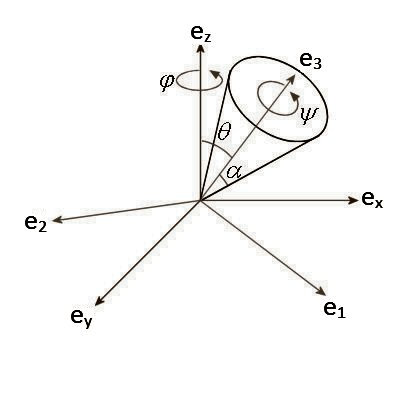
\includegraphics[height=4cm]{tuoluo1.jpg}
 \caption{拉格朗日陀螺示意图}
\end{figure}
\par 此外,我们记陀螺对$\textbf{e}_1,\textbf{e}_2,\textbf{e}_3$的转动惯量分别为$I_1,I_2,I_3$,由于陀螺对称,我们有
$$I_1=I_2=I\neq I_3 $$
另记陀螺在$\textbf{e}_1,\textbf{e}_2,\textbf{e}_3$方向的角速度分别为$\omega_1,\omega_2,\omega_3$.角速度与欧拉角之间的关系如下
$$\omega_1=\dot{\theta},\omega_2=\dot{\phi}\sin \theta,\omega_3=\dot{\psi} + \dot{\phi}\cos \theta ,$$
陀螺对于轴$i$的角动量$M_i,(i=1,2,3)$可以表示为$M_i=I_i\omega_i,(i=1,2,3)$.
我们可以将该运动的动能表述为:
 $$T= \frac{1}{2}I(\dot{\theta}^{2} + \dot{\phi}^{2}\sin^{2}\theta) + \frac{1}{2}I_{3}\left( \dot{\psi} + \dot{\phi}\cos \theta\right)^{2}$$
 相应的势能为$V = Mgl\cos \theta$.这里$l$是陀螺质心到固定点$O$在铅直方向的距离.
 总的拉格朗日函数为:
 $$L = \frac{1}{2}I(\dot{\theta}^{2} + \dot{\phi}^{2}\sin^{2}\theta) + \frac{1}{2}I_{3}\left( \dot{\psi} + \dot{\phi}\cos\theta\right)^2-Mgl\cos\theta .$$
\par 我们的推导从这里开始,容易发现拉格朗日函数里不显含$\phi,\psi$于是有:
 \begin{align*}
 \frac{\partial L}{\partial \phi} = 0 \Rightarrow
 \frac{d}{dt}\frac{\partial L}{\partial \dot{\phi}} = 0 \Rightarrow
 p_{\phi} = \frac{\partial L}{\partial \dot{\phi}} = \text{const}\\
  \frac{\partial L}{\partial \psi} = 0 \Rightarrow
 \frac{d}{dt}\frac{\partial L}{\partial \dot{\psi}} = 0 \Rightarrow
 p_{\psi} = \frac{\partial L}{\partial \dot{\psi}} = \text{const}.
 \end{align*}
 通过诺特定理一节的例\ref{jdl}我们知道旋转不变性对应的守恒量为角动量,所以这里$p_{\psi},p_{\phi}$就是角动量$M_3,M_z$
 我们现在来计算角动量$p_{\psi}$和$p_{\phi}$:
$$p_{\psi} = \frac{\partial L}{\partial \dot{\psi}} = I_{3}\left(\dot{\psi} + \dot{\phi}\cos \theta \right) = \text{const} \text{,}$$
而角动量$p_{\psi}$又可以表示成$p_{\psi}=I_3\omega_3$,由此$\omega_3$是常数.我们定义常数$a = \frac{I_{3}}{I}\omega_{3}$.
对于$p_{\phi}$,我们也有:
$$p_{\phi} = \frac{\partial L}{\partial \dot{\phi}} =I\dot{\phi}\sin^{2}\theta + I_{3}\left( \dot{\psi}+\dot{\phi}\cos\theta\right)\cos\theta =\text{const} \text{,}$$
定义另一个常数$b = \frac{p_{\phi}}{I}$,通过下面两个关系式我们可以看出$a,b$的联系.
\begin{align*}
p_{\psi} &= aI = I_{3}\left( \dot{\psi} + \dot{\phi}\cos\theta
\right)\\
    b &= \frac{p_{\phi}}{I} = \dot{\phi}\sin^{2}\theta +
\frac{I_{3}}{I}\left( \dot{\psi} + \dot{\phi}\cos\theta
\right)\cos\theta\\
\Rightarrow b&= \dot{\phi}\sin^{2}\theta + a\cos \theta .
\end{align*}
我们可以进一步将$\dot{\phi}$表示为$\theta$的函数:
$$\dot{\phi}=\frac{b - a\cos \theta}{\sin^{2}\theta}$$
我们还有一个守恒量是系统的总能量$E$,它可以表示为:
$$E = T+ V = \frac{I}{2}\left( \dot{\theta}^{2} +\dot{\phi}^{2}\sin^{2}\theta \right) + \frac{I_{3}}{2}\omega_{3}^{2}+ Mgl\cos\theta = \text{const} $$
注意$\frac{I_{3}}{2}\omega_{3}^{2}$也是一个常数,我们记$E^{\prime}=E-\frac{I_{3}}{2}\omega_{3}^{2}$则
$$E^{\prime}=\frac{I}{2}\left( \dot{\theta}^{2} +\dot{\phi}^{2}\sin^{2}\theta \right)+ Mgl\cos\theta = \text{const} ,$$
而$\dot{\phi}=\frac{b - a\cos \theta}{\sin^{2}\theta}$
于是
$$E^{\prime}\frac{I}{2}\dot{\theta}^{2} +\frac{I}{2}\frac{\left( b - a\cos \theta \right)^{2}}{\sin^{2}\theta}+mgl\cos\theta = \text{const}$$
定义有效势能$V\text{eff}(\theta) = \frac{I}{2}\frac{\left( b - a\cos \theta \right)^{2}}{\sin^{2}\theta}+mgl\cos\theta $,
原问题被化作了一个关于$\theta$的一维问题,且有方程
$$\dot{\theta} = \frac{d\theta}{dt} = \sqrt{\frac{2}{I}\left( E' -V\text{eff}(\theta) \right)},$$
对时间$t$求解有
$$t(\theta) = \int_{}^{}\frac{d\theta}{\sqrt{\frac{2}{I}\left(E'-V\text{eff}(\theta) \right)}}$$
这是一个椭圆积分且可以被积出来,但我们的目标是得到$\theta(t)$.
\par 观察$V\text{eff}$,我们发现当$\theta$接近$0$或$\pi$时,$V\text{eff}$会增大,但$V\text{eff}$需要小于$E'$,这给$\theta$的大小增加了限制,易知$\theta$在其最大最小值之间周期变化,其临界值由$V\text{eff}=E'$给出.
\par 为了求解这个这个问题,我们做变量代换$(u = \cos \theta)$,
计算$\dot{u}$以将$E'$表示为$E'(u,\dot{u})$.
$$\dot{u} = -\sin \theta\dot{\theta} \Rightarrow\dot{\theta}^{2} = \frac{\dot{u}^{2}}{\sin^{2}\theta}, \sin^{2}\theta = 1 - \cos^{2}\theta = 1 - u^{2},$$
将结果代回$E'$并乘以$(\sin^{2}\theta)$
\begin{align*}
    E'\sin^{2}\theta &= \frac{1}{2}\dot{\theta}^{2}\sin^{2}\theta +
    \frac{I}{2}\left( b - a\cos \theta \right)^{2} + mgl\cos \theta
    \sin^{2}\theta\\
    E'(1 - u^{2}) &= \frac{I}{2}\dot{u}^{2} + \frac{I}{2}\left( b - au
\right)^{2} + mglu(1 - u^{2}).
\end{align*}
定义新常数:$\alpha = \frac{2E'}{I}, \beta = \frac{2mgl}{I}$,
将上面关于$E'$的表达乘以$(\frac{2}{I})$,我们有
\begin{align*}
\alpha(1 - u^{2}) = \dot{u}^{2} + (b - au)^{2}+\beta u(1 - u^{2}),
\end{align*}
将$\dot{u}^{2}$放在方程一边并记$f(u)=(1 - u^{2})(\alpha - \beta u) - (b - au)^{2}$,
则关于$E'$的能量守恒律变为$\dot{u}^{2}=f(u)$.
注意$f(u)$是关于$u$的三次多项式,且$(-1 \leq u \leq 1)$,为了研究$f(u)$的根,取极限:
\begin{align*}
u \rightarrow \infty &\Rightarrow f(u) \rightarrow \beta u^{3}
\rightarrow + \infty\\
u \rightarrow -\infty &\Rightarrow f(u) \rightarrow -\beta u^{3}
\rightarrow -\infty
\end{align*}
另外有$f(\pm1)=-(a\mp b)^2<0$当$a\neq \pm b$,则当$f(u)$的极大值大于1时,方程有三个实根,否则只有一个实根,且当只有一个实根时$|u|>1$.于是实际运动对应的常数$a,b,\alpha,\beta$会使方程的两个根$u_1,u_2$落在$[-1,1]$区间,这样可以根据$u_1,u_2$确定$\theta$ 变化范围区间$[\theta_1,\theta_2]$,陀螺轴倾角的变化称为陀螺的章动.
\begin{figure}[h]
 \renewcommand{\captionfont}{\small}
 \centering
 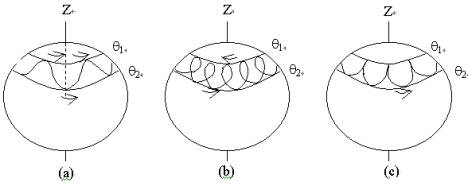
\includegraphics[height=3.5cm]{tuoluo.jpg}
 \caption{陀螺的进动与章动}
 \end{figure}
\par 现在回到式子$\dot{\phi}=\frac{b - a\cos \theta}{\sin^{2}\theta}$,$\phi$表示陀螺轴方位角的变化,称为陀螺的进动或者岁差.考虑陀螺轴在单位圆周上画出的曲线,它的变化有以下几种情况:
\begin{itemize}
 \item [(1)]$b > a \Rightarrow \dot{\phi} > 0$:陀螺倾角在$\theta_{1}$,$\theta_{2}$之间变化,进动沿着同一方向进行转轴在单位球面上画出正弦曲线.(图2(a))
 \item [(2)]$b < a \Rightarrow \dot{\phi} \lessgtr 0 $:如果$b < a $,$\dot{\phi}$有可能随着$\cos \theta$改变,轨迹在单位圆一侧画出一串带圈曲线.(图2(b))
 \item [(3)]$b - a\cos \theta_{1} = 0 \Rightarrow\theta_{1} = \cos^{-1}\left( \frac{b}{a} \right)$:当$\theta = \theta_{1}$ 时刻没有进动,单位圆
 一侧轴的轨迹像是一系列重复在最高点相连接的抛物线.(图2(c))
 \end{itemize}
 \par 陀螺的运动由其绕自身轴的旋转,章动和进动决定,三者有各自的频率,当三者频率不通约时,陀螺永远不会回到其起始点,但可以任意接近它.\cite{AI3}
\par 地球绕地轴旋转,可以看做是一个巨大的陀螺.由于受到太阳等其他星球的万有引力,会产生垂直于转轴方向的力矩分量,也就是说地球的自转轴并不是始终指向一个方向,而是会产生绕着黄道轴的进动.当地球自转轴旋进时,春分点西移,地球公转不到360$^{\circ}$即可两次经过春分点,恒星年和回归年便产生了一个差值,这就是岁差.公元前二世纪,古希腊天文学家喜帕恰斯在编制一本包含1022颗恒星的星表时,首次发现了岁差现象.中国晋代天文学家虞喜,根据对冬至日恒星的中天观测,独立地发现了岁差.据《宋史$\cdot$律历志》记载:“虞喜云:‘尧时冬至日短星昴,今二千七百余年,乃东壁中,则知每岁渐差之所至'”.岁差这个名词即由此而来.
\newpage
\section{哈密顿力学}
\subsection{哈密顿方程}
\subsubsection{勒让德变换}
本节我们首先用勒让德变换从拉格朗日方程推导出哈密顿方程.
\begin{dfn}
让$f:\mathbf{R}^n\rightarrow\mathbf{R}$为一凸函数,也即其Hessian矩阵$\nabla^2f$正定.则函数$f$的勒让德变换为:$\mathcal{L}(f)(p)=max_x(p\textbf{x}-f(\textbf{x}))$
\end{dfn}
勒让德变换将关于$\mathbf{x}$ 的函数$f$变为一个关于新的独立变量$\textbf{p}$ 的函数.其变换步骤如下:首先引入新的独立变量$\textbf{p}$,构造函数$F(\textbf{x},\textbf{p})=\textbf{p}\cdot \textbf{x}-f(\textbf{x})$;此时假定$\textbf{p}$ 为一给定值,然后让$\textbf{x}$ 取值为$\textbf{x}(\textbf{p})$,以使函数$F(\textbf{x},\textbf{p})$ 在该$\textbf{p}$ 值之下达到最大值.这样我们就得到了关于$\textbf{p}$ 的函数$g(\textbf{p})=\mathcal{L}(f)(\textbf{p})=\textbf{p}\cdot \textbf{x}(\textbf{p})-f(\textbf{x}(\textbf{p}))=max_x(\textbf{p}\cdot \textbf{x}-f(\textbf{x}))$.
\begin{thm}
凸函数$f(\textbf{x})$经过勒让德变换后得到的函数$g(\textbf{p})$仍为凸函数,且勒让德变换具有对合性:$\mathcal{L}(\mathcal{L}(f))(\textbf{x})=f(\textbf{x})$.
\end{thm}
\begin{pf}
令$g(\textbf{p})=\mathcal{L}(f)(\textbf{p})$,关于变量$\textbf{p}$ 求其梯度,得
$$\nabla g(\textbf{p})=\textbf{p}\cdot (\nabla \textbf{x})(\textbf{p})+\textbf{x}(\textbf{p})-(\nabla f)(\textbf{x}(\textbf{p}))\cdot (\nabla \textbf{x})(\textbf{p})=\textbf{x}(\textbf{p}).$$
这里$\textbf{x}(\textbf(p))$依定义要使$F(\textbf{x},\textbf{p})$ 在相应的$\textbf{p}$ 下达到最大值.在$F(\textbf{x},\textbf{p})=\textbf{p}\cdot \textbf{x}-f(\textbf{x})$ 中,固定$\textbf{p}$,让它对$\textbf{x}$ 求梯度为$\textbf{0}$,可以发现$\textbf{x}(\textbf(p))$ 即为方程$\textbf{p}-\nabla (f)(\textbf{x})=\textbf{0}$ 的解.
利用上面的讨论,下面首先证明凸函数经勒让德变换后仍为凸函数.
如果$g(\textbf{p})=\mathcal{L}(f)(\textbf{p})$,那么
\begin{align*}
\nabla^2g(\textbf{p})&=\nabla(\textbf{x}(\textbf{p}))\\
&=\nabla{\textbf{x}[(\nabla f)(\textbf{x}(\textbf{p}))]}\\
&=(\nabla \textbf{x})[(\nabla f)(\textbf{x}(\textbf{p}))]\cdot(\nabla^2 f)(\textbf{x}(\textbf{p}))\cdot(\nabla \textbf{x})(\textbf{p})\\
&=(\nabla \textbf{x})(\textbf{p})\cdot (\nabla^2 f)(\textbf{x}(\textbf{p}))\cdot(\nabla \textbf{x})(\textbf{p})
\end{align*}
正定,所以$g(\textbf{p})$也为凸函数.\\
\par 接下来我们证明勒让德变换的对合性.
我们要计算的是$\mathcal{L}(g)(\textbf{x})=\mathcal{L}(\mathcal{L}f(\textbf{x}))(\textbf{x})$ 这里的$\textbf{x}$是我们在函数$g(\textbf{p})$上引入的新变量,
为了避免混淆,我们将函数$g(\textbf{p})=\textbf{p}\cdot \textbf{x}(\textbf{p})-f(\textbf{x}(\textbf{p}))$ 改记为
$g(\textbf{p})=\textbf{p}\cdot y(\textbf{p})-f(y(\textbf{p}))$.
新记号下根据之前所述,$y(\textbf{p})$满足条件$\textbf{p}=(\nabla f)(y(\textbf{p}))$,
且$(\nabla g)(\textbf{p})=y(\textbf{p})$.
在变换$\mathcal{L}(g)(\textbf{x})=\textbf{x}\cdot \textbf{p}-g(\textbf{p})$ 中,根据勒让德变换定义,固定$\textbf{x}$,
$\textbf{p}(\textbf{x})$应该使$\textbf{x}\cdot \textbf{p}-g(\textbf{p})$ 最大,
则$\textbf{p}(\textbf{x})$应满足$\textbf{x}-(\nabla g)(\textbf{p}(\textbf{x}))=\mathbf{0}$,
那么有:
\begin{align*}
\mathcal{L}(g)(\textbf{x})&=\textbf{x}\cdot \textbf{p}(\textbf{x})-g(\textbf{p}(\textbf{x}))\\
&=(\nabla g)(\textbf{p}(\textbf{x}))\cdot \textbf{p}(\textbf{x})-g(\textbf{p}(\textbf{x}))\\
&=y(\textbf{p}(\textbf{x}))\cdot \textbf{p}(\textbf{x})-[\textbf{p}(\textbf{x})\cdot y(\textbf{p}(\textbf{x}))-f(y(\textbf{p}(\textbf{x})))]\\
&=f(y(\textbf{p}(\textbf{x})))=f(\textbf{x})
\end{align*}
即证
\end{pf}
我们刚才给出的证明是用的代数方法,阿诺德在\cite{AI4}中用几何方法证明了这点.他的证明基于这样一个事实:如果$g(p)=\mathcal{L}(f)(p)\text{那么}y=xp-g(p)\text{是}y=f(x)\text{在}x(p)\text{点}\text{的斜率为}p$的切线.
\subsubsection{哈密顿方程的导出}
\begin{thm}
拉格朗日方程\eqref{Eq:EL}等价于哈密顿方程:
\begin{equation}
\dot{\textbf{p}}=-\frac{\partial H}{\partial \dot{\textbf{q}}}\text{,} \dot{\textbf{q}}=\frac{\partial H}{\partial \dot{\textbf{p}}} \label{Eq:H}
\end{equation}
这里哈密顿函数$H(p,q,t)$为$\mathcal{L}(L_{q,t})(\dot{q})$,即对拉格朗日函数关于$\dot{q}$进行勒让德变换(把$q,t$视作参数)后得到的函数.
\end{thm}
\begin{pf}
我们从拉格朗日方程\eqref{Eq:EL}入手.由勒让德变换的定义,$H(\textbf{p})=\textbf{p}\cdot \dot{\textbf{q}}-L(\dot{\textbf{q}})\text{,这里} \textbf{p}=\partial L/\partial \dot{\textbf{q}}$,这样我们可以把$\dot{\textbf{q}}$ 表示为$\textbf{p}$的函数.注意到$H$也是$\textbf{q},t$的函数.我们先计算$H$ 关于$\textbf{p}$ 和$\textbf{q}$ 的偏导数:
$$\frac{\partial H}{\partial \textbf{p}}=\dot{\textbf{q}}+\textbf{p}\cdot \frac{\dot{\textbf{q}}}{dp}-\frac{\partial L}{\partial \dot{\textbf{q}}}\cdot\frac{d\dot{\textbf{q}}}{d\textbf{p}}=\dot{\textbf{q}}$$
$$\frac{\partial H}{\partial \textbf{q}}=-\frac{\partial L}{\partial \textbf{q}}=-\dot{\textbf{p}}$$
如此得到了哈密顿方程,这里第二个等式可以由拉格朗日方程直接推出.
\par 然后我们再来从哈密顿方程推导拉格朗日方程.这里需要用到勒让德变换的对合性.
假设哈密顿方程\eqref{Eq:H}成立,将它看做$\textbf{p}$ 的函数,对其运用勒让德变换得:$L(\dot{\textbf{q}})=\dot{\textbf{q}}\cdot \textbf{p}-H(\textbf{p})$,这里$\dot{\textbf{q}}$为引入的新变量
$\textbf{p}$满足$\dot{\textbf{q}}=\partial H/\partial \textbf{p}$.由哈密顿方程,$\partial H/\partial \textbf{p}=\frac{d}{dt}\textbf{q}$,所以$\dot{\textbf{q}}$ 确实是关于时间的导数.现在对$L$关于$\textbf{p},\textbf{q}$ 分别求偏导数:
$$\frac{\partial L}{\partial \textbf{q}}=-\frac{\partial H}{\partial \textbf{q}}=\dot{\textbf{p}}$$
$$\frac{\partial L}{\partial \dot{\textbf{q}}}=\textbf{p}+\dot{\textbf{q}}\cdot\frac{d\mathbf{p}}{d\dot{\textbf{q}}}-\frac{\partial H}{\partial \textbf{p}}\frac{d\mathbf{p}}{d\dot{\textbf{q}}}=\textbf{p}$$
两个式子结合起来就是拉格朗日方程\eqref{Eq:EL}. 两者的等价性得证.
\end{pf}
虽然哈密顿方程组与拉格朗日方程组等价,但它在某些方面更具优势.首先哈密顿方程组对称的一阶偏微分方程组,从这种方程形式上比身为二阶偏微分方程组的拉格朗日方程组简单.而且我们后面会看到,哈密顿方程容许的坐标变换比拉格朗日方程组更多.
\begin{thm}
如果可以将拉格朗日函数$L$表示为$T-U$的形式,这里$T=1/2\sum a_{ij}(\textbf{q},t)\dot{q}^i\dot{q}^j$是一个关于广义坐标的二次型,$U=U(\textbf{q})$.
在该假设下哈密顿函数即总能量:$H=T+U$.
\end{thm}
\begin{pf}
我们首先要证明对二次型$f=\sum f_{ij}x^ix^j$应用勒让德变换得到函数$g(p)$,$f(\textbf{x})$与$g(\textbf{p}(\textbf{x}))$ 在对应点处所得值相等.这是因为
\begin{align*}
\nabla f(\textbf{x})\cdot \mathbf{x}&=(\sum\limits_if_{ij}x^j+\sum\limits_jf_{ij}x^i)\cdot\sum\limits_ix^i\\
&=\sum\limits_i\sum\limits_jf_{ij}x^jx^i+\sum\limits_i\sum\limits_jf_{ij}x^ix^j\\
&=2\sum\limits_{ij}f_{ij}x^ix^j=2f(\textbf{x})
\end{align*}
由此$g(\textbf{p})=\textbf{p}\textbf{x}-f(\textbf{x})=\nabla f(\textbf{x})\cdot\textbf{x}-f(\textbf{x})=2f(\textbf{x})-f(\textbf{x})=f(\textbf{x})$\\
同理可得
$$H=\textbf{p}\dot{\textbf{q}}-L=\frac{\partial L}{\partial \dot{\textbf{q}}}-L=\frac{\partial T}{\partial \dot{\textbf{q}}}-L=2T-(T-U)=T+U$$
即证.
\end{pf}
\begin{cor}
在同样假设下,若力学系的哈密顿量不显含时间,则能量守恒:$\frac{dH}{dt}=\frac{\partial H}{\partial t}$.
\end{cor}
\begin{pf}
哈密顿量是关于$(\textbf{p},\textbf{q},t)$的函数
\begin{align*}
\frac{dH}{dt}&=\frac{\partial H}{\partial \textbf{p}}\dot{\textbf{p}}+\frac{\partial H}{\partial \textbf{q}}\dot{\textbf{q}}+\frac{\partial H}{\partial t}\\
&=-\frac{\partial H}{\partial \textbf{p}}\frac{\partial H}{\partial \textbf{q}}+\frac{\partial H}{\partial \textbf{q}}\frac{\partial H}{\partial \textbf{p}}+\frac{\partial H}{\partial t}\\
&=\frac{\partial H}{\partial t}.
\end{align*}
\end{pf}
要说明的是哈密顿量是否等于体系总能量与能量是否守恒这是两个完全不同的问题,如果$\partial H/\partial t$ 那么它只说明哈密顿量不守恒,但能量$E$可能守恒,它不一定等于$H$.
在哈密顿力学里我们可以同样的定义循环坐标的概念,且易知坐标$q_i$ 为哈密顿 函数的循环坐标当且仅当它是拉格朗日函数的循环坐标.我们之前证明的诺特定理可以推广到哈密顿系统里,相应的对称性指变换保持哈密顿函数不变.对于$\frac{\partial H}{\partial q_i}=0$,我们依然可以得出相应方向的广义动量守恒:$p_i=const$.我们同样可以通过寻找守恒律来减少系统自由度,简化系统的求解.本章最后一节提到的正则变换给了我们寻找守恒量的另一种方法.


\subsection{正则变换}
在相空间里我们用$2n$个独立变量描述系统的状态,有时候某组特定的坐标(比如一组全为循环坐标的坐标)比之其他坐标能更方便的描述这个系统,此时我们需要进行坐标变换$(\textbf{p},\textbf{q})\rightarrow (\textbf{P}(\textbf{p},\textbf{q}),\textbf{Q}(\textbf{p},\textbf{q}))$.为了让这个变换是有效的,我们还需要对变换增加一些限制.首先我们要求这个变换至少在局部上是可逆的,这样如果我们求出$(\textbf{P}(t),\textbf{Q}(t)$后还能从它推出$(\textbf{p}(t),\textbf{q}(t))$.更重要的是,我们希望哈密顿方程在新坐标下仍有相同的形式.自然地,我们想要用数学语言刻画出满足以上要求的变换的特征,上节讲到的辛形式能帮我们做到这一点.
\begin{dfn}
令$g$为相空间$\mathbf{R}^{2n}={(\textbf{p},\textbf{q})}$到$\textbf{R}^{2n}$的可微映射.映射$g$称为正则变换,如果$g$保持2-形式$\omega^2=\sum dp_i\wedge dq_i$不变:$g^*\omega^2=\omega^2$.
\end{dfn}
上节的定理\ref{bx}也可以叙述为相流在相空间里给出正则变换.
本节我们首先证明正则变换保持哈密顿方程的形式,然后给出部分正则变换的例子,最后以一个一维简谐振荡的例子结束.
证明正则变换保持哈密顿方程的形式前,我们要介绍一些概念.
\par 首先取扩充的相空间$M(p_1,\ldots,p_n,q_1,\ldots,q_n,t)$.对于偶数维流形$M^{2n}$上的2-形式$\omega$我们称它为非奇异的如果它的特征值不含零,对于奇数维的流形$M^{2n+1}$上的2-形式$\omega$,我们称它为非奇异的如果它只有一个特征值为零.现在我们假设$\omega$为$M^{2n+1}$上的一个1-形式,且$d\omega$非奇异,则在$M^{2n+1}$ 上的每一点都有一个$d\omega$的零化方向,称为涡方向.沿着涡方向积分会得到涡线.对于$M^{2n+1}$上的一条闭合曲线$\gamma$,从$\gamma$每一点出发都可以得到一条涡线,这些涡线合起来构成了涡管. 现在我们在扩展的相空间$M^{2n+1}$ 里给定一个函数$H=H(\textbf{p},\textbf{q},t)$,我们作1-形式
$$\omega^1=\textbf{p}d\textbf{q}-Hdt(\textbf{p}d\textbf{q}=p_1dq_1+\ldots+p_ndq_n),$$
我们要对它证明如下引理.
\begin{lem}\label{pv}
$2n+1$维扩充相空间$\textbf{p},\textbf{q},t$上的形式$\omega^1=\textbf{p}d\textbf{q}-Hdt$之涡线在$t$轴上有一对一的投影,即可表示为函数$\textbf{p}(t),\textbf{q}(t)$.这些函数满足以$H$为哈密顿函数的正则方程组:
\begin{equation}
\frac{d\textbf{p}}{dt}=-\frac{\partial H}{\partial \textbf{q}},\frac{d\textbf{q}}{dt}=\frac{\partial H}{\partial \textbf{p}} \label{Eq:H3} .
\end{equation}
也就是说,1-形式$\textbf{p}d\textbf{q}-Hdt$的涡线是相流在扩充相空间中的轨道,即上述正则方程组的积分曲线.
\end{lem}
\begin{pf}
对$\omega^1$微分有
$$d\omega^1=\omega^2=\sum\limits_{i=1}^n(dp_i\wedge{d}q^i-\frac{\partial{H}}{\partial{q^i}}dq^i\wedge{d}t-\frac{\partial{H}}{\partial{p_i}}dp_i\wedge{d}t),$$
由此可见2-形式$\omega^2$在坐标$(\textbf{p},\textbf{q},t)$下的矩阵为
$$\left(\begin{array}{ccc}
 0   & -I_n & H_p \\
 I_n &   0  & H_q \\
-H_p & -H_q & 0
\end{array}\right).$$
注意到左上角$2n\times2n$的子矩阵满秩,而矩阵本身为奇数阶反对称阵,所以其行列式为零,那么矩阵的秩就是$2n$,于是矩阵的核的维数为1,进而$\omega^1$非奇异,可以验证$(-\nabla_{\textbf{q}}H,\nabla_{\textbf{p}}H,1)$即为相应的零化向量,也就是说$(-\nabla_{\textbf{q}}H,\nabla_{\textbf{p}}H,1)$给出了$\omega^1$涡线的方向.
另一方面,$(-\nabla_{\textbf{q}}H,\nabla_{\textbf{p}}H,1)$也是扩充相空间内相流的切向量.所以相流的轨道就是1-形式$\omega^1$的涡线.
\end{pf}
1-形式$\textbf{p}d\textbf{q}-Hdt$也叫做庞加莱积分不变量,历史上它来自讨论与讨论路径光学长度的作用量函数\cite{AI8}.
我们下面来证明本节的主要的定理.
\begin{thm}
正则变换保持哈密顿方程的形式
\end{thm}
\begin{pf}
由正则变换定义,在新坐标系下辛形式$\sum dP_i\wedge dQ_i$与旧坐标系下辛形式$\sum dp_i\wedge dq_i$相同.于是有
$$d(\textbf{p}d\textbf{q}-\textbf{P}d\textbf{Q})=d\textbf{p}\wedge d\textbf{q}-d\textbf{P}\wedge d\textbf{Q}=0.$$
显然1-形式$\textbf{p}d\textbf{q}-\textbf{P}d\textbf{Q}$为闭形式.注意我们现在讨论的底空间是在$\textbf{R}^{2n}$有第一章中对闭形式和恰当形式的讨论,我们知道在欧氏空间中闭形式就是恰当形式.于是存在函数$S:\textbf{R}^{2n}\rightarrow \textbf{R}$使得$\textbf{p}d\textbf{q}-\textbf{P}d\textbf{Q}=dS$.于是存在1-形式
$$\omega^1=\textbf{p}d\textbf{q}-Hdt=\textbf{P}d\textbf{Q}-Hdt+dS.$$
让函数$K:\textbf{R}^{2n}\rightarrow \textbf{R}$定义为$K(\textbf{P},\textbf{Q})=H(\textbf{P}(\textbf{p},\textbf{q}),\textbf{Q}(\textbf{p},\textbf{q}))$.
由于$ddS=0$在新旧坐标下对$\omega^1$微分有
$$d\omega^1=d\textbf{p}\wedge d\textbf{q}-dH\wedge dt=d\textbf{P}\wedge d\textbf{Q}-dK\wedge dt.$$
$\omega^1$的涡方向由$d\omega^1$的零化方向给出,由于对$\textbf{p}d\textbf{q}-Hdt$和$\textbf{P}d\textbf{Q}-Kdt$微分得到的2-形式相同,所以两者有相同的涡线.
由引理\ref{pv},新坐标系下$\textbf{P},\textbf{Q}$满足的方程形式与旧坐标系下,即相同的哈密顿量$K=H$下的哈密顿方程.
\end{pf}
下面引入生成函数概念帮助我们构造正则变换.我们可以从刚才的证明知道如果$2n$个变量$\textbf{p},\textbf{q}$的$2n$个函数$\textbf{P}(\textbf{p},\textbf{q}),
\textbf{Q}(\textbf{p},\textbf{q})$给出正则变换$g:\textbf{R}^{2n}\rightarrow \textbf{R}^{2n}$,则1-形式$\textbf{p}d\textbf{q}-\textbf{P}d\textbf{Q}$是全微分:
\begin{equation}
\textbf{p}d\textbf{q}-\textbf{P}d\textbf{Q}=dS(\textbf{p},\textbf{q}) \label{Eq:sc}
\end{equation}
可以证明若此1-形式是全微分,则变换是正则变换\cite{AI10}.
\par 现在设在某点$(\textbf{p}_0,\textbf{q}_0)$附近可取$(\textbf{Q},\textbf{q})$为独立坐标,也即其雅可比行列式在$(\textbf{p}_0,\textbf{q}_0)$点不为零:
$$det\frac{\partial (\textbf{Q},\textbf{q})}{\partial (\textbf{p},\textbf{q})}\big|_{\textbf{p}_0,\textbf{q}_0}=det\frac{\partial \textbf{Q}}{\partial \textbf{p}}\big|_{\textbf{p}_0,\textbf{q}_0} \neq 0 .$$
此时正则变换称为自由的,此时函数可以局部的用新坐标表示:
$$S(\textbf{p},\textbf{q})=F_1(\textbf{Q},\textbf{q}) .$$
\begin{dfn}
上面给出的函数$F_1(\textbf{Q},\textbf{q})$称为正则变换$g$的(第一类)生成函数.
\end{dfn}
这里$F_1$是$\textbf{R}_{\textbf{q}}^n\times\textbf{R}_{\textbf{Q}}^n$中的某个区域的函数,且根据定义知$F_1$的偏导数为
$$\frac{\partial F_1(\textbf{Q},\textbf{q})}{\partial \textbf{q}}=\textbf{p} \text{和}\frac{\partial F_1(\textbf{Q},\textbf{q})}{\partial \textbf{Q}}=-\textbf{P} .$$
由$F_1$可以给出自由的正则变换.由$F_1$还可以构造出非自由正则变换的生成函数,具体见\cite{AI9},我们将常用的四类生成函数总结如下:
\begin{table}[h]
\renewcommand{\captionfont}{\small}
\begin{center}

	\caption{常用生成函数类}
	\vskip 4mm

	\begin{tabular}{c|c|c|c}
    \text{类型} & \text{函数} & \text{偏导数} & \text{示例}\\ \hline
1 & \( F_{1}(q, Q, t) \) & \( \begin{array}{l}
p_{i} = \frac{\partial F_{1}}{\partial q_{i}} \\
 P_{i} = -\frac{\partial F_{1}}{\partial Q_{i}}
\end{array}   \)
 & \( \begin{array}{l}
 F_{1}  = q_{i}Q_{i}\\
Q_{i} = p_{i}\\
P_{i} = -q_{i}
\end{array} \)\\ \hline
2 & \( F_{2}(q, Q, t) \) &
\( \begin{array}{l}
    p_{i} = \frac{\partial F_{2}}{\partial q_{i}}\\
 P_{i} = \frac{\partial F_{2}}{\partial Q_{i}}
 \end{array} \)
 &
 \( \begin{array}{l}
 F_{2}  = q_{i}P_{i}\\
Q_{i} = q_{i}\\
P_{i} = p_{i}
\end{array} \)\\ \hline
3 & \( F_{3}(q, Q, t) \) &
\( \begin{array}{l}
p_{i} = -\frac{\partial F_{3}}{\partial q_{i}}\\
P_{i} = -\frac{\partial F_{3}}{\partial Q_{i}}
\end{array} \)
& \(
\begin{array}{l}
    F_{3}  = q_{i}Q_{i}\\
Q_{i} = -q_{i}\\
P_{i} = -p_{i}
\end{array} \)\\ \hline
4 & \( F_{4}(q, Q, t) \) & \(
\begin{array}{l}
    p_{i} = -\frac{\partial F_{4}}{\partial q_{i}}\\
P_{i} = \frac{\partial F_{4}}{\partial Q_{i}}
\end{array} \)
& \(
\begin{array}{l}
    F_{4}  = p_{i}P_{i}\\
Q_{i} = p_{i}\\
P_{i} = -q_{i}
\end{array}\)
\end{tabular}\end{center}\end{table}

事实上拉格朗日力学中对于广义坐标的变换就是一种正则变换,称作点变换,它可以由第二类生成函数数生成.由此可以看到,哈密顿方程容许的变换比拉格朗日方程更多,这也是哈密顿表述相比于拉格朗日表述的优势之一.
\par 下面给出一个通过正则变换得到循环坐标的例子.
\begin{exmp}
考虑一维简谐振子的运动,该运动的哈密顿函数可表示为$H= \frac{1}{2m}\left( p^{2} + m^{2}\omega^{2}q^{2} \right)$,我们想用正则变换使变换后的坐标$\textbf{Q}$ 成为循环坐标.尝试如下变换:
\begin{align*}
p = f(P)\cos\left( Q \right) \qquad q =
\frac{f(P)}{m\omega}\sin\left( Q \right)
\end{align*}
变换后的哈密顿函数变为$K = H = \frac{f(P)^{2}}{2m}$.显然$Q$成为了循环坐标.
\par 我们需要找到$f(P)$的显式表达.这里套用第一类生成函数
\begin{align*}
F_{1}(q ,Q,t) \qquad p = \frac{\partial F_1}{\partial q} \qquad P =
-\frac{\partial F_1}{\partial Q}
\end{align*}
将$p$写成$(q,Q)$的函数有$p = m\omega q \cot (Q) = \frac{\partial F_1}{\partial q}$.于是
$$F_1 = \frac{m\omega q^{2}}{2}\cot (Q)$$
进一步的我们可以得到$P$的显式表达,
$$P = -\frac{\partial F}{\partial Q} = \frac{m\omega q^{2}}{2}\frac{1}{\sin^{2}\left( Q \right)},$$
由此有
$$q(Q, P) = \sqrt{\frac{2P}{m\omega}}\sin(Q) \Rightarrow f(P)=\sqrt{2m\omega P}.$$
则$K=\omega P$,现在我们可以列出新坐标下的正则方程
$$\dot{P}= -\frac{\partial K}{\partial Q}=0 \qquad \dot{Q}=\frac{\partial K}{\partial P}=\omega.$$
由此解得$q(t)=\sqrt{\frac{2E}{m\omega^2}}\sin(\omega t+Q(0))$.这里$E$是系统总能量.
\end{exmp}
这里举一维谐振子的例子是因为谐振子问题是经典力学中的基本问题.任何体系在平衡位置附近的振动在适当的坐标变换之后,都可以分解为若干彼此独立的谐振动.此外,谐振子在量子力学中的也有重要应用可用于分析分子的振动,晶格的振动,原子核表面振动以及辐射场的振动等等.这里提到量子力学是因为哈密顿量在量子力学中也有重要应用.哈密顿方程的对称性为它在量子力学和统计力学等领域中的应用提供了理论基础,换言之,哈密顿理论为我们提供了一个方便推广到更多物理领域的理论框架,为我们从经典力学过度到量子力学提供了便利.

\newpage
\section{总结与未来工作展望}
以阿诺德的《经典力学的数学方法》为基础,本文用数学语言简要介绍了牛顿力学,拉格朗日力学以及哈密顿力学中的大部分重要概念和定理.着重体现了三种力学相空间的差异,以及这种差异带来的研究方法的不同.此外突出了系统对称性与守恒量之间的联系以及如何运用守恒量减少问题自由度,简化问题的求解.此外,本文在原书基础上补充了一些证明,或者将某些证明从一维推广到高维.
\par 未来研究方向包括以下几点:第一,本文研究的系统多为自治系统,可研究非自制系统下的方程性质,并将资质条件下定义定理推广到非自制情形;第二,本文提到的约束都为完整约束,可研究非完整约束下的情形;第三,本文限于篇幅对哈密顿力学提及较少,可深化对哈密顿系统以及相关的辛几何学的学习;第四,本文大部分在做定性描述,未来可研究哈密顿方程以及哈密顿雅可比方程的数值求解.
\newpage
%% TODO: bibliography
%下面修改参考文献格式
\makeatletter
\renewenvironment{thebibliography}[1]
{\section*{\refname}%
\@mkboth{\MakeUppercase\refname}{\MakeUppercase\refname}%
\list{\@biblabel{\@arabic\c@enumiv}}%
{\settowidth\labelwidth{\@biblabel{#1}}%
\leftmargin\labelwidth
\advance\leftmargin\labelsep
\advance\leftmargin by 0em%   %设置文本距离左边距距离
\itemindent 0em%    %设置编号后内容缩进
\@openbib@code
\usecounter{enumiv}%
\let\p@enumiv\@empty
\renewcommand\theenumiv{\@arabic\c@enumiv}}%
\sloppy
\clubpenalty4000
\@clubpenalty \clubpenalty
\widowpenalty4000%
\sfcode`\.\@m}
{\def\@noitemerr
{\@latex@warning{Empty `thebibliography' environment}}%
\endlist}
\makeatother

\addcontentsline{toc}{section}{参考文献}
\begin{thebibliography}{MM}
\addtolength{\itemsep}{-0.5em}% TODO:
\begin{small}
\bibitem{AI1} Arnold V I. Mathematical methods of classical mechanics[M]. Springer, 1989: 4-6.
\bibitem{drm} Robbin J W, Salamon D A. Introduction to differential topology[J]. UW Madison, ETH Zürich, 2011:49-99.
\bibitem{CL} Cornelius Lanczos. The variational principles of mechanics[M]. Courier Dover Publications, 1970.
\bibitem{zzs} 张筑生.\ 微分拓扑新讲[M].\ 北京大学出版社, \ 2002.
\bibitem{css} Chern S S. Lecture note on differential geometry[J]. Chicago Univ, 1950.
\bibitem{AI2} Arnold V I. Mathematical methods of classical mechanics[M]. Springer, 1989: 82.
\bibitem{CL1} Cornelius Lanczos. The variational principles of mechanics[M]. Courier Dover Publications, 1970: 180-190.
\bibitem{AI3} Arnold V I. Mathematical methods of classical mechanics[M]. Springer, 1989: 152-158.
\bibitem{AI4} Arnold V I. Mathematical methods of classical mechanics[M]. Springer, 1989: 63.
\bibitem{zzs1} 张筑生.\ 微分拓扑新讲[M].\ 北京大学出版社, \ 2002: 157-160.
\bibitem{AI11} Arnold V I. Mathematical methods of classical mechanics[M]. Springer, 1989: 71.
\bibitem{AI5} Arnold V I. Mathematical methods of classical mechanics[M]. Springer, 1989: 163-200.
\bibitem{AI6} Arnold V I. Mathematical methods of classical mechanics[M]. Springer, 1989: 178.
\bibitem{AI7} Arnold V I. Mathematical methods of classical mechanics[M]. Springer, 1989: 206-207.
\bibitem{AI8} Arnold V I. Mathematical methods of classical mechanics[M]. Springer, 1989: 263.
\bibitem{AI10} Arnold V I. Mathematical methods of classical mechanics[M]. Springer, 1989: 258.
\bibitem{AI9} Arnold V I. Mathematical methods of classical mechanics[M]. Springer, 1989: 266-270.
\bibitem{AI} Arnold V I. Mathematical methods of classical mechanics[M]. Springer, 1989: 204-206.
\bibitem{AIc} Arnold V I, Kozlov V V, Neitadt A I. Mathematical aspects of classical and celestial mechanics[M]. Springer-Vlg, 1985.
\bibitem{bf} Sarlet W, Cantrijn F. Generalizations of Noether's theorem in classical mechanics[J]. Siam Review, 1981, 23(4): 467-494.
\bibitem{ld} Landau L D, EM Lifshitz. Mechanics: Volume 1 (Course Of Theoretical Physics)[J]. Butterwor, 1976.
\bibitem{gd} Goldstein H, Poole C, Safko J, et al. Classical mechanics[J]. American Journal of Physics, 2002, 70: 782-783.
\bibitem{gd2} Goldstein H. Classical mechanics[M]. Pearson Education India, 1962.
\bibitem{zxk} 张贤科, 许甫华.\ 高等代数学[M].\ 清华大学出版社有限公司,\ 2004.
\bibitem{EM} Gross D, Hauger W, Schruder J, et al. Engineering Mechanics 3: Dynamics[M]. Springer, 2011.

\bibitem{1}  库恩. 科学革命的结构:第四版[M].金吾伦,胡新和,译.2 版.北京:北京大学出版社,2012:25.
\bibitem{2}何晓群,刘文卿. 应用回归分析[M]. 北京: 中国人民大学出版社,   2011:107-110.
\bibitem{3}魏浩.  股票价格影响因素分析[J].  企业研究. 2012,18: 34-35.
\bibitem{4}赵国顺.  基于时间序列分析的股票价格趋势预测研究[D]. 厦门: 厦门大学, 2009.
\bibitem{5} 戴军,黄志文,葛新元.  Logistic选股模型及其在沪深300中的实证[EB/OL]. (2010-09-07)[2016-5-28].  http://www. doc88.com/p-3187558973748.html.



\end{small}
\end{thebibliography}
%\end{CJK*}
\newpage
\section*{谢\quad 辞}
\addcontentsline{toc}{section}{谢\quad 辞}
%章节不标号时用\section*{},并用\addcontentsline{toc}{section}{}将其加入目录
谢辞内容
\end{document}
